\begin{frame}
	\frametitle{Código repetido}

	\begin{figure}[h]
		\centering
			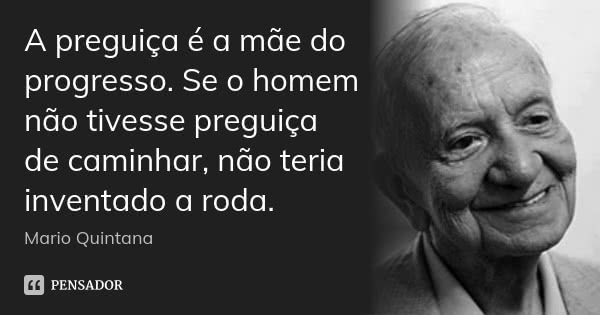
\includegraphics[height=0.6\paperheight]{figuras/mario}
		\caption{Retirada do site \href{https://www.pensador.com/frase/MTY2/}{Pensador}}\label{figure:mario}
	\end{figure}

\end{frame}


\begin{frame}
	\frametitle{Problemas}

	\begin{itemize}
		\item Dificulta a manutenção
		\item As funções podem ser diferentes
		\item Dificuldade de localizar o problema
		\item As vezes não é tão eficiênte
	\end{itemize}

\end{frame}

\begin{frame}
	\Huge Caso real
\end{frame}

\begin{frame}[fragile]
	\frametitle{Classe \textit{Form\char`_GerenciarAcomodacoes}}

	\begin{minted}[baselinestretch=1.2,fontsize=\scriptsize,linenos]{csharp}
//Função para validar as strings (não permitir caracteres especiais)
public bool validaStr(string str)
{
	Regex r = new Regex("^[a-zA-ZáéíóúàèìòùâêîôûãõçÁÉÍÓÚÀÈÌÒÙÂÊÎÔÛÃÕÇ0-9 -]*$");
    return r.IsMatch(str);
}
\end{minted}

\end{frame}

\begin{frame}[fragile]
	\frametitle{Classe \textit{Form\char`_GerenciarFuncionario}}

	\begin{minted}[baselinestretch=1.2,fontsize=\scriptsize,linenos]{csharp}
//Função para validar as strings (nao permitir caracteres especiais)
public bool validaStr(string str)
{
	Regex r = new Regex("^[a-zA-ZáéíóúàèìòùâêîôûãõçÁÉÍÓÚÀÈÌÒÙÂÊÎÔÛÃÕÇ -]*$");
    return r.IsMatch(str);
}
	\end{minted}

\end{frame}

\begin{frame}[fragile]
	\frametitle{Classe \textit{Form\char`_GerenciarTarifas}}

	\begin{minted}[baselinestretch=1.2,fontsize=\scriptsize,linenos]{csharp}
//Função para validar as strings (nao permitir caracteres especiais)
public bool validaStr(string str)
{
	Regex r = new Regex("^[a-zA-ZáéíóúàèìòùâêîôûãõçÁÉÍÓÚÀÈÌÒÙÂÊÎÔÛÃÕÇ0-9 -]*$");
    return r.IsMatch(str);
}
	\end{minted}

\end{frame}

\begin{frame}

	\Huge Elas eram iguais?

\end{frame}

\begin{frame}
	\Huge Exemplo
\end{frame}

\begin{frame}[fragile]
	\frametitle{Função para substituir vogais por espaço}

	\begin{minted}[baselinestretch=1.2,fontsize=\scriptsize,linenos]{c}
bool substituirVogaisPorEspaco(char *string){
	char vogais[]="aeiouAEIOU";
	bool substituiu = false;

	for( int i=0; i<strlen(string); i++){
		for( int j=0; j<strlen(vogais); j++){
			if(string[i] == vogais[j]){
				string[i] = ' ';
				substituiu = true;
			}
		}
	}

	return substituiu;
}
	\end{minted}

\end{frame}

\begin{frame}[fragile]
	\frametitle{Função para substituir números pela letra A}

	\begin{minted}[baselinestretch=1.2,fontsize=\scriptsize,linenos]{c}
bool substituirNumerosPorLetras(char *string){
	char numeros[]="0123456789";
	bool substituiu = false;

	for( int i=0; i<strlen(string); i++){
		for( int j=0; j<strlen(numeros); j++){
			if(string[i] == numeros[j]){
				string[i] = 'A';
				substituiu = true;
			}
		}
	}

	return substituiu;
}
	\end{minted}

\end{frame}

\begin{frame}[fragile]
	\frametitle{NOVA Função para substituir vogais por espaço}

	\begin{minted}[baselinestretch=1.2,fontsize=\scriptsize,linenos]{c}
bool substituirVogaisPorEspaco(char *string){
	char vogais[] = "aeiouAEIOU";

	bool substituiu = false, tmp;

	for( int i=0; i<strlen(vogais); i++){
		tmp = substituirCaractere(string, vogais[i], ' ');
		if(tmp){
			substituiu = tmp;
		}
	}

	return substituiu;
}
	\end{minted}

\end{frame}

\begin{frame}[fragile]
	\frametitle{NOVA Função para substituir números pela letra A}

	\begin{minted}[baselinestretch=1.2,fontsize=\scriptsize,linenos]{c}
bool substituirNumerosPorLetras(char *string){
	char numeros[]="0123456789";

	bool substituiu = false, tmp;

	for( int i=0; i<strlen(numeros); i++){
		tmp = substituirCaractere(string, numeros[i], 'A');
		if(tmp){
			substituiu = tmp;
		}
	}

	return substituiu;
}
	\end{minted}

\end{frame}

\begin{frame}[fragile]
	\frametitle{NOVA Função para substituir caracteres}

	\begin{minted}[baselinestretch=1.2,fontsize=\scriptsize,linenos]{c}
bool substituirCaractere(char *string, char antigoCaractere, char novoCaractere){
	bool substituiu = false;

	for( int i=0; i<strlen(string); i++){
		if(string[i] == antigoCaractere){
			string[i] = novoCaractere;
			substituiu = true;
		}
	}

	return substituiu;
}
	\end{minted}

\end{frame}

\begin{frame}
	\frametitle{Solução}

	\begin{itemize}
		\item Remover a repetição e reorganizar
	\end{itemize}

\end{frame}
